\let\negmedspace\undefined
\let\negthickspace\undefined
\documentclass[journal]{IEEEtran}
\usepackage[a5paper, margin=10mm, onecolumn]{geometry}
%\usepackage{lmodern} % Ensure lmodern is loaded for pdflatex
\usepackage{tfrupee} % Include tfrupee package

\setlength{\headheight}{1cm} % Set the height of the header box
\setlength{\headsep}{0mm}     % Set the distance between the header box and the top of the text

\usepackage{gvv-book}
\usepackage{gvv}
\usepackage{cite}
\usepackage{amsmath,amssymb,amsfonts,amsthm}
\usepackage{algorithmic}
\usepackage{graphicx}
\usepackage{textcomp}
\usepackage{xcolor}
\usepackage{txfonts}
\usepackage{listings}
\usepackage{enumitem}
\usepackage{mathtools}
\usepackage{gensymb}
\usepackage{comment}
\usepackage[breaklinks=true]{hyperref}
\usepackage{tkz-euclide} 
\usepackage{listings}
% \usepackage{gvv}                                        
\def\inputGnumericTable{}                                 
\usepackage[latin1]{inputenc}                                
\usepackage{color}                                            
\usepackage{array}                                            
\usepackage{longtable}                                       
\usepackage{calc}                                             
\usepackage{multirow}                                         
\usepackage{hhline}                                           
\usepackage{ifthen}                                           
\usepackage{lscape}
\usepackage{circuitikz}
\tikzstyle{block} = [rectangle, draw, fill=blue!20, 
    text width=4em, text centered, rounded corners, minimum height=3em]
\tikzstyle{sum} = [draw, fill=blue!10, circle, minimum size=1cm, node distance=1.5cm]
\tikzstyle{input} = [coordinate]
\tikzstyle{output} = [coordinate]


\begin{document}

\bibliographystyle{IEEEtran}
\vspace{3cm}

\title{2.7.8}
\author{EE25BTECH11026-Harsha}
 \maketitle
% \newpage
% \bigskip
{\let\newpage\relax\maketitle}

\renewcommand{\thefigure}{\theenumi}
\renewcommand{\thetable}{\theenumi}
\setlength{\intextsep}{10pt} % Space between text and floats


\numberwithin{equation}{enumi}
\numberwithin{figure}{enumi}
\renewcommand{\thetable}{\theenumi}

\textbf{Question}:\\
    Find $|\vec{a}-\vec{b}|$, if two vectors $\vec{a}$ and $\vec{b}$ are such that $|\vec{a}|=2$,$|\vec{b}|=3$ and $\vec{a}.\vec{b}=4$.\\ 
\solution \\
Let us solve the given equation theoretically and then verify the solution computationally.\\
\\
According to the question,\\
\begin{align}
    |\vec{a}|=2 \;\; ; \; |\vec{b}|=3 \;\; ;\; \vec{a}^T\vec{b}=4
\end{align}
The  value of $\|\vec{a}-\vec{b}\|$ can be computed by the following formula,
\begin{align}
    \|\vec{a}-\vec{b}\|^2=\|\vec{a}\|^2+\|\vec{b}\|^2-2\vec{a}^T\vec{b}
\end{align}
\begin{align}
    \therefore \|\vec{a}-\vec{b}\|^2=2^2+3^2-2\times4
\end{align}
\begin{align}
    \|\vec{a}-\vec{b}\|^2=5
\end{align}
\begin{align}
    \implies \|\vec{a}-\vec{b}\|=\sqrt{5}=2.2361 units
\end{align}
From the figure, taking an example of vectors $\vec{a}$ and $\vec{b}$ ,it is clearly verified that the theoretical solution matches with the computational solution.\\
\begin{figure}[H]
    \centering
    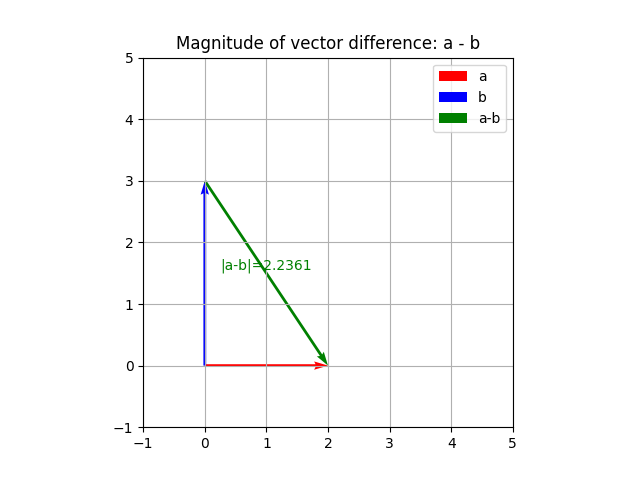
\includegraphics[width=0.6\columnwidth]{figs/Figure_1.png}
    \label{fig-1}
\end{figure}



 


\end{document}